\subsection{UCW3 - Creazione grafico}
\label{sub:ucw3}

\begin{figure}[h]
    \centering
    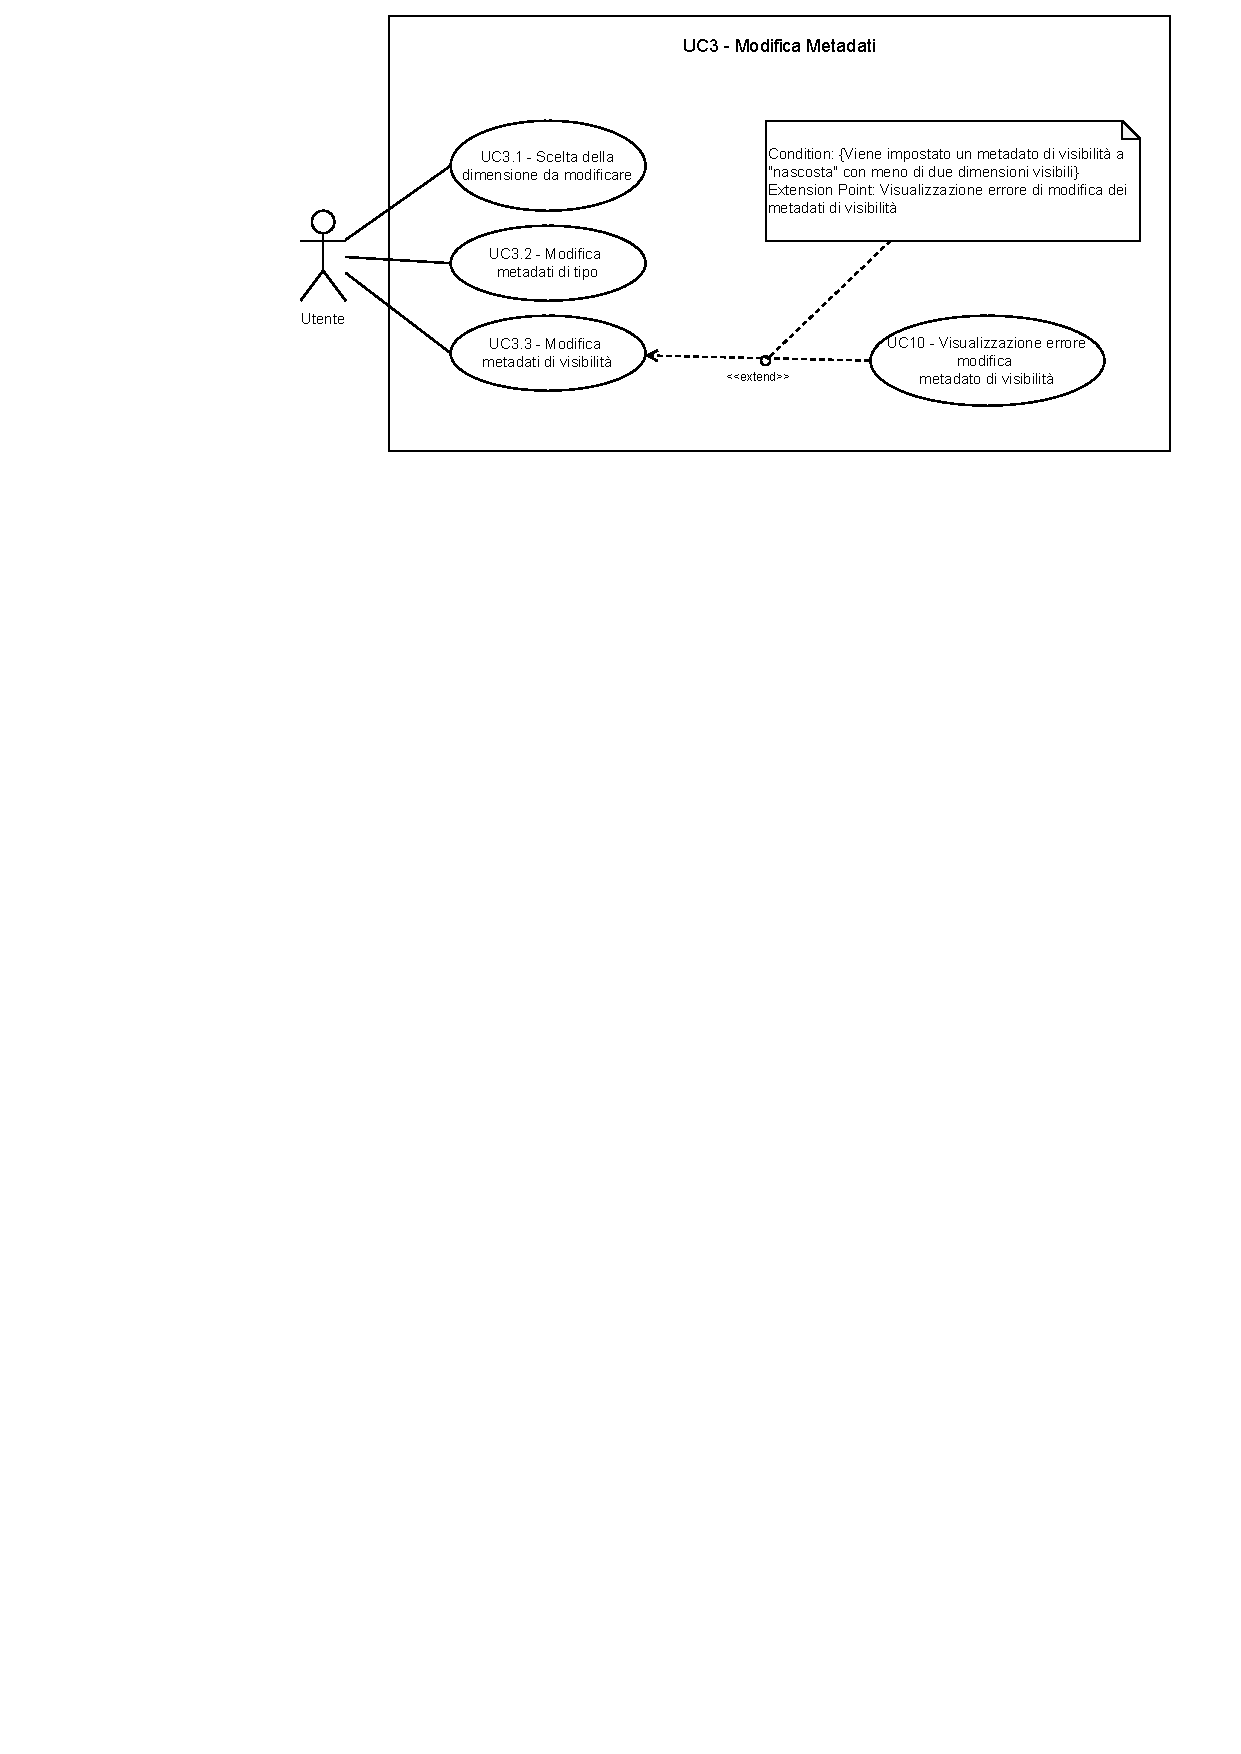
\includegraphics[width=0.8\textwidth]{diagrammi/UC3.pdf}
    \caption{Diagramma rappresentante UCW3}
    \label{fig:UCW3}
\end{figure}


\begin{itemize}
	\item \textbf{Descrizione}: L’utente seleziona dal menù di creazione di un grafico una tipologia di 
	visualizzazione, viene poi computato il relativo grafico mediante i dati caricati e infine visualizzato;
	
    \item \textbf{Attore primario}: Utente;
    
    \item \textbf{Precondizione}: É stato creato un ambiente valido (\hyperref[sub:ucs1]{UCS1});

	\item \textbf{Postcondizione}:  Viene visualizzato il grafico della tipologia scelta dall'utente a partire dai dati 
	correntemente presenti nell'ambiente; 

	\item \textbf{Scenario principale}:
		\begin{enumerate}
			\item L'utente seleziona l'opzione che desidera tra le tipologie di grafico (\hyperref[ssub:ucw3.1]{UCW3.1});
			\item Il sistema calcola il grafico della tipologia selezionata sui dati precedentemente caricati;
			\item Il sistema visualizza il grafico computato.
		\end{enumerate}
\end{itemize}

\subsubsection{UCW3.1 - Selezione grafico}
\label{ssub:ucW3.1}
\begin{itemize}

	\item \textbf{Descrizione}: L’utente seleziona la tipologia di grafico che desidera costruire;

    \item \textbf{Attore primario}: Utente;

	\item \textbf{Precondizione}:   É stato creato un ambiente valido (\hyperref[sub:ucs1]{UCS1});
	
    \item \textbf{Postcondizione}:  É stata selezionata la tipologia del grafico che verrà costruito;

	\item \textbf{Generalizzazioni}:
		\begin{enumerate}
			
			\item Selezione di Scatterplot matrix \hyperref[ssub:ucw3.2]{UCW3.2};
			\item Selezione di Force Field \hyperref[ssub:ucw3.3]{UCW3.3};
			\item Selezione di Heat Map \hyperref[ssub:ucw3.4]{UCW3.4};
			\item Selezione di Proiezione Lineare Multiasse \hyperref[ssub:ucw3.5]{UCW3.5};
			\item Selezione di Distance Map \hyperref[ssub:ucw3.6]{UCW3.6}.
			
		\end{enumerate}

\end{itemize}


\subsubsection{UCW3.2 - Selezione di Scatter Plot Matrix}
\label{ssub:ucw3.2}
\begin{itemize}

	\item \textbf{Descrizione}: L’utente seleziona \emph{Scatter Plot Matrix} come tipologia di grafico che desidera 
	costruire, visualizzando le prime 5 dimensioni considerando l'ordimento nel dataset;

    \item \textbf{Attore primario}: Utente;

	\item \textbf{Precondizione}:   É stato creato un ambiente valido (\hyperref[sub:ucs1]{UCS1});

	\item \textbf{Postcondizione}:  L'utente ha selezionato \emph{Scatter Plot Matrix} come tipologia del grafico da 
	costruire;

	\item \textbf{Scenario Principale}:
	\begin{enumerate}
		\item L'utente seleziona \emph{Scatter Plot Matrix} come tipologia di grafico da costruire.
	\end{enumerate}
\end{itemize}


\subsubsection{UCW3.3 - Selezione di Force Field}
\label{ssub:ucw3.3}
\begin{itemize}

	\item \textbf{Descrizione}: L’utente seleziona \emph{Force Field} come tipologia di grafico che desidera 
	costruire utilizzando la distanza euclidea su tutte le dimensioni del dataset;

    \item \textbf{Attore primario}: Utente;

    \item \textbf{Precondizione}:   É stato creato un ambiente valido (\hyperref[sub:ucs1]{UCS1});

    \item \textbf{Postcondizione}:  L'utente ha selezionato \emph{Force Field} come tipologia del grafico da 
	costruire;
	
	\item \textbf{Scenario Principale}: 
	\begin{enumerate}
		\item L'utente seleziona \emph{Force Field} come tipologia del grafico da costruire.
	\end{enumerate}

\end{itemize}


\subsubsection{UCW3.4 - Selezione di Heat Map}
\label{ssub:ucw3.4}
\begin{itemize}

	\item \textbf{Descrizione}: L’utente seleziona \emph{Heat Map} come tipologia di grafico che desidera 
	costruire, con un gradiente di default;

    \item \textbf{Attore primario}: Utente;

	\item \textbf{Precondizione}:   É stato creato un ambiente valido (\hyperref[sub:ucs1]{UCS1});

    \item \textbf{Postcondizione}:  L'utente ha selezionato \emph{Heat Map} come tipologia del grafico da 
	costruire;

	\item \textbf{Scenario Principale}: 
	\begin{enumerate}
		\item L'utente seleziona \emph{Heat Map} come tipologia del grafico da costruire.
	\end{enumerate}

\end{itemize}


\subsubsection{UCW3.5 - Selezione di Proiezione Lineare Multi Asse}
\label{ssub:ucw3.5}
\begin{itemize}

	\item \textbf{Descrizione}: L’utente seleziona \emph{Proiezione Lineare Multi Asse} come tipologia di grafico che 
	desidera costruire, visualizzando le prime 2 dimensioni considerando l'ordimento nel dataset;

    \item \textbf{Attore primario}: Utente;

    \item \textbf{Precondizione}:   É stato creato un ambiente valido (\hyperref[sub:ucs1]{UCS1});

	\item \textbf{Postcondizione}:  L'utente ha selezionato \emph{Proiezione Lineare Multi Asse} come tipologia del 
	grafico da costruire;
	
	\item \textbf{Scenario Principale}: 
	\begin{enumerate}
		\item L'utente seleziona \emph{Proiezione Lineare Multi Asse} come tipologia del grafico da costruire.
	\end{enumerate}
\end{itemize}

\subsubsection{UCW3.6 - Selezione di Distance Map}
\label{ssub:ucw3.6}
\begin{itemize}
	\item \textbf{Descrizione}: L’utente seleziona \emph{Distance Map} come tipologia di grafico che desidera 
	costruire con un gradiente di default;
	\item \textbf{Attore primario}:	Utente;
	\item \textbf{Precondizione}:	É stato creato un ambiente valido (\hyperref[sub:ucs1]{UCS1});

    \item \textbf{Postcondizione}:  L'utente ha selezionato \emph{Distance Map} come tipologia del grafico da 
	costruire;

	\item \textbf{Scenario Principale}: 
	\begin{enumerate}
		\item L'utente seleziona \emph{Distance Map} come tipologia del grafico da costruire.
	\end{enumerate}
\end{itemize}
